\scanpage{7}
d'un $\unsure{\underline\Gamma}$]. Formellement, [de façon précise : à cela près qu'on a des pro-Modules au lieu de Modules tt courts] on voit que $Q^0[M]$ est un (pro)Module stratifié sur $X$ rel $S$, et les $Q^i[M]$ sont les composantes du (pro)Module \deleted{\unsure{$Q$}} cosimplicial correspondant.
\margin{\figure{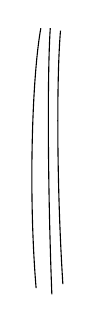
\begin{tikzpicture}[x=1cm,y=1cm]
\draw (0,0) .. controls (-.10,1.2) and (-.05,2.7) .. (.06,3.3);
\draw (.20,-.08) .. controls (.15,1.2) and (.14,2.7) .. (.18,3.3);
\draw (.34,.05) .. controls (.26,1.3) and (.26,2.7) .. (.31,3.27);
\end{tikzpicture}}}

Ce pro-Module stratifié $Q^0[M]$, \inserted{des parties principales} dépend fonctoriellement de $M$ parcourant $\operatorname{Mod}(X/S)$ [Modules sur $X$ avec op. diff. \inserted{rel $S$} d'\uline{\deleted{\unsure{un}}\inserted{ordre} borné}], en prenant comme hom de pro-objets ceux au sens de Artin-Riesz.
De plus, on récupère $M$ à partir de $Q^0[M]$ [pro-objet à stratification] comme étant le sous-faisceau des \uline{sections stationnaires} [\unsure{dans la structure}
\margin{\figure{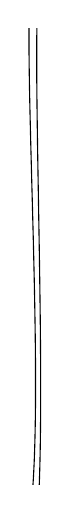
\begin{tikzpicture}[x=1cm,y=1cm]
\draw (0,0) .. controls (.10,1.5) and (-.06,4.4) .. (-.05,5.8);
\draw (.08,0) .. controls (.14,1.6) and (.03,4.5) .. (.05,5.8);
\end{tikzpicture}}}
\margin{6}
